\documentclass{article}

% Document extensibility %
%
% Disables native paragraph indentation
\usepackage{parskip} 
%
% Provides further bullet options for lists
\usepackage{enumitem}

% Mathematical symbol and statement packages %
%
% Necessary
\usepackage{amsmath}
\usepackage{amssymb}
%
% Extensive fraction notation
\usepackage{xfrac}
%
% Generic mathematical commands
% Notable: \degree, \celcius
\usepackage{gensymb}
%
% Variable vector notation (arrow above variable)
\usepackage{esvect}
%
% Multiline boxed equations
\usepackage{empheq}
\usepackage{siunitx}

% Graphic packages %
%
% Diagrams and illustrations
\usepackage{tikz}
\usetikzlibrary{angles, quotes, positioning, calc}
%
% Image insertion
\usepackage{graphicx}

% Document content %
%
% Change title of table of contents
% \renewcommand{\contentsname}{Title}

\begin{document}

% Command `\hr` to insert horizontal rules
\newcommand{\hr}{\par\noindent\rule{\textwidth}{0.4pt}}

\tableofcontents
\newpage

\section{Lesson 4}

% \subsection{Practice Problem}
% 
% Two blocks, $ A $ and $ B $, are placed as shown, and connected by cords to block $ C $. $ A $ and $ B $ weigh $ 20 $ lb. each, and the coefficient of sliding friction between each block and the surface is $ 0.5 $. Block $ C $ descends with constant velocity.
% 
% \begin{tikzpicture}
%     \tikzstyle{block} = [draw=black, thick, align=center, rectangle]
% 
%     \draw[very thick, black, ->] (0, 0) -- (5, 0) node [right] {$+\hat{x}$};
% 
%     \draw[thick, black] (2, 0) node (A) {}
%         -- (4, 2) node [midway] (B) {}
%         -- (4, 0) node (C) {};
%     \draw pic["$\theta$", draw=orange, thick, angle radius=1cm, ->] {angle = C--A--B};
% 
%     \node[block, above=0cm of B, rotate=45] (Bblock) {B};
%     \draw[block] (1, 0) node (ABlock) {A};
% \end{tikzpicture}

\subsection{Center of Mass}

\textbf{Center of Mass}: average location of mass in a distribution
\begin{itemize}[label=-]
    \item Balance Point
    \item Natural Rotation axis
    \item Only line through center of mass on a 2D object always splits into 2 equal parts
\end{itemize}
A center of mass for point masses can be given by the equation
$$ \vec{x}_{\text{CM}} = \frac{\vec{\sum}m_i\vec{x}_i}{\sum m_i} $$
In one-dimension
$$ x_{\text{CM}} = \frac{\sum m_ix_i}{m_{\text{total}}} $$

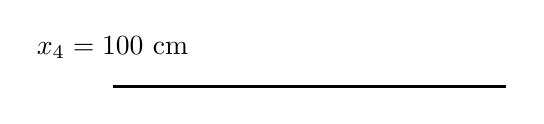
\begin{tikzpicture}
    \draw[very thick, black] (0, 0) node (start) {} -- (5, 0) node (end) {};

    \node (10/5/5, 0) (x1) {};
    \node (50/5/5, 0) (x2) {};
    \node (70/5/5, 0) (x3) {};
    \node ($ 100/5/5 $, 0) (x4) {};

    % \node[above=0.1cm of x1] {$x_1=10$ cm};
    % \node[above=0.1cm of x2] {$x_2=50$ cm};
    % \node[above=0.1cm of x3] {$x_3=70$ cm};
    \node[above=0.1cm of x4] {$x_4=100$ cm};
\end{tikzpicture}

If you have a vector equation then find their components and handle them separately.

\begin{align*}
    P_1 & = (3, 3) \\
    m_{P_1} & = \SI{27}{\kg} \\
    P_2 & = (0, 0) \\
    m_{P_2} & = \SI{10}{\kg} \\
    P_3 & = (-1, 1) \\
    m_{P_3} & = \SI{9}{\kg} \\
    P_4 & = (-4, -2) \\
    m_{P_4} & = \SI{15}{\kg}
\end{align*}
First finding the $ x $ components
\begin{align*}
    x_1 & = \SI{3}{\m} \\
    m_1 & = \SI{27}{\kg} \\
    x_2 & = \SI{0}{\m} \\
    m_2 & = \SI{10}{\kg} \\
    x_3 & = \SI{-1}{\m} \\
    m_3 & = \SI{9}{\kg} \\
    x_4 & = \SI{-4}{\m} \\
    m_4 & = \SI{15}{\kg}
\end{align*}
Then the $ y $ components
\begin{align*}
    y_1 & = \SI{3}{\m} \\
    m_1 & = \SI{27}{\kg} \\
    y_2 & = \SI{0}{\m} \\
    m_2 & = \SI{10}{\kg} \\
    y_3 & = \SI{1}{\m} \\
    m_3 & = \SI{9}{\kg} \\
    y_4 & = \SI{-2}{\m} \\
    m_4 & = \SI{15}{\kg}
\end{align*}
Then solving for $ x_{CM} $
\begin{align*}
    x_{CM} & = \frac{\sum m_ix_i}{m_{\text{total}}} \\
           & = \frac{(\SI{3}{\m})(\SI{27}{\kg}) + (\SI{0}{\m})(\SI{10}{\kg}) + (\SI{-1}{\m})(\SI{9}{\kg}) + (\SI{-4}{\m})(\SI{15}{\kg})}{\SI{27}{\kg} + \SI{10}{\kg} + \SI{9}{\kg} + \SI{15}{\kg}} \\
           & = \SI{0.2}{\m}
\end{align*}

\begin{align*}
    y_{CM} & = \frac{ (\SI{3}{\m}\SI{27}{\kg}) + (\SI{0}{\m}\SI{10}{\kg}) + (\SI{1}{\m}\SI{9}{\kg}) + (\SI{-2}{\m}\SI{15}{\kg}) }{ \SI{27}{\kg} + \SI{10}{\kg} + \SI{9}{\kg} + \SI{15}{\kg} } \\
    & = \SI{1}{\m}
\end{align*}

\subsection{Density}

\textbf{Density}: $ \frac{\text{amount}}{\text{space it takes up}} $

Volumetric mass density
$$ \rho \equiv \frac{dm}{dV} $$
For continuous solids instead of $ \sum m_ix_i $ we use
$$ \int x dm $$
Because $ dm $ is hard to work with we say
$$ dm = \rho dV $$
A \textbf{moment} is defined by
$$ \int x\rho dV $$
Where $ \rho dV $ shows integrating with respect to space

Counting moments is $ 0 $-indexed

Zeroth moment
\begin{align*}
    & \int x^0\rho dV \\
    & = \int\rho dV \\
    & = \int_0^{M_\text{total}}dm \\
    & = M_{\text{total}}
\end{align*}
First moment
\begin{align*}
    & \int x^1\rho dV \\
    & = \int x\rho dV \text{, related to torque}
\end{align*}
Center of Mass:
$$ \vec{x}_{\text{CM}} = \frac{\int \vec{x}\rho dV}{\int \rho dr} $$
Given the general function for $ y $ of $ x $
$$ y = -\frac{h}{b}x + h $$
\begin{align*}
    M_{\text{total}}\vec{x}_{\text{CM}} & = \sum x\sigma dA \\
                        & = \int (x)\sigma(ydx) \\
                        & = \sigma \int_0^b x(-\frac{h}{b}x + h)dx \\
                        & = \sigma \int_0^b \left(-\frac{h}{b}x^2 + hx\right)dx \\
                        & = \sigma \left(-\frac{h}{3b}x^3 + \frac{h}{2}x^2\right)_0^b
\end{align*}

\end{document}
